\subsection{CIFAR-10 Dataset}
The CIFAR-10 dataset is a subset of the 80 million tiny images. They were collected by Alex Krizhevsky, Vinod Nair, and Geoffrey Hinton.//
The CIFAR-10 dataset consists of 60000 32x32 color images in 10 classes, with 6000 images per class. There are 50000 training images and 10000 test images.//
The dataset is divided into five training batches and one test batch, each with 10000 images. The test batch contains exactly 1000 randomly-selected images from each class. The training batches contain the remaining images in random order, but some training batches may contain more images from one class than another. Between them, the training batches contain exactly 5000 images from each class. The sample from CIFAR-10 dataset is given in Figure \ref{cifar10}.

\begin{figure}[h!]
  \centering
  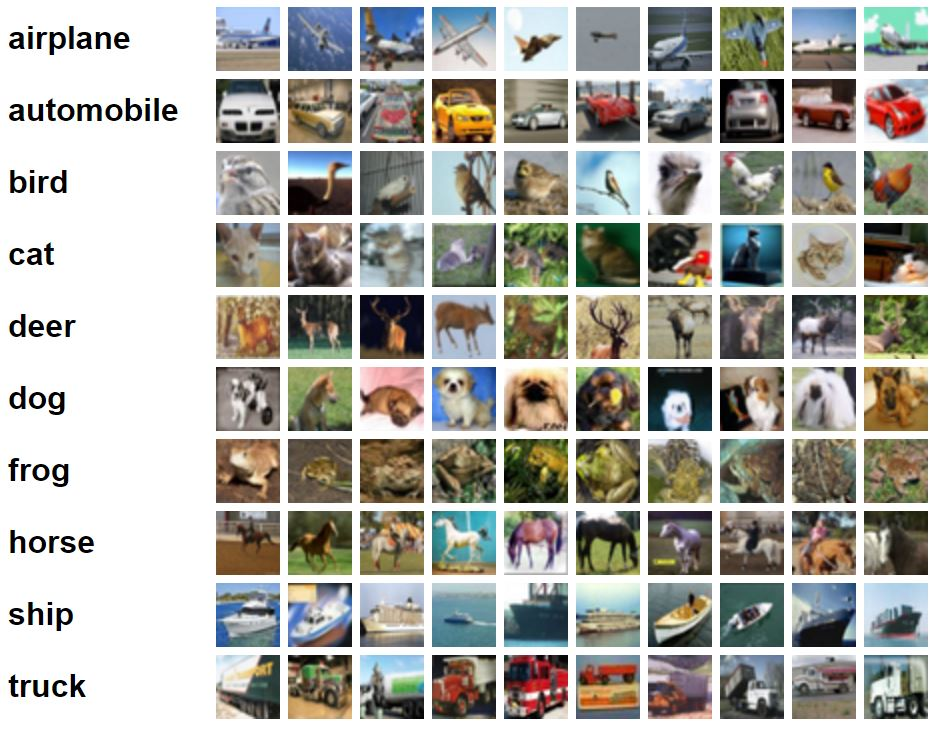
\includegraphics[width=.4\textwidth]{images/cifar10.JPG}
  \caption{CIFAR-10 Dataset} \label{cifar10}
  \vspace{-.5cm}
\end{figure}

\subsection{Multi Label Dataset}
As we are using single label dataset(CIFAR-10) for our single label Convolutional Neural Network, we have to use images that contain the identical contents from CIFAR-10. So, we picked random 100 images containing the identical contents as CIFAR-10 and tested it with our model. For an example, from Figure \ref{multi} we see that the image contains only a cat and a  dog, which our Single Label Convolutional Network can classify. So, the images we chose only contains subset of airplane, automobile, bird, cat, deer, dog, frog, horse, ship, truck.  

\begin{figure}[h!]
  \centering
  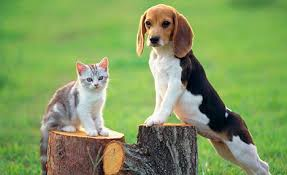
\includegraphics[width=.3\textwidth]{images/multi.jpg}
  \caption{Multi Label Image} \label{multi}
  \vspace{-.5cm}
\end{figure}